\section{Body Chapter: Segmentation and Glossing}
\label{sec:seggls}

%Morphological analysis of a language begins with identifying, segmenting, and glossing morphemes in words. Only a small percentage of tokens in transcribed text contain unusual and interesting morphological forms. Thus, a large chunk of this highly time-consuming work is as monotonous to the annotator as it is uninformative to language science. It can and should be assisted by machine learning. 
The study proposed in this section asks: \emph{How do choices made during interlinearization (i.e. surface versus canonical segmentation, in/consistent morpheme boundaries, lack/presence of part of speech tags) affect machine learning results on morpheme segmentation and glossing?} The experiments will compare three machine learning models for segmenting and glossing when trained on two different segmentation strategies. They will be conducted on four languages that have been manually segmented with surface and canonical strategies. 
%Segmentation and glossing lays the foundation for further morphological analysis and description so 
%This study will also determine the best models to be used in the second study (Section \ref{sec:balance}). 
The experiments will address two questions.

\begin{enumerate}
    \item To what extent do segmentation choices affect the performance of a neural Transformer model compared to a Conditional Random Fields model? 
    \item Is a segment-then-gloss sequential approach ever preferable over joint learning of morpheme segments and glosses?
\end{enumerate}
    
\subsection{Segmentation Strategies}    
Each machine learning system will be trained, tested, and compared on both (surface) morphs and (canonical) morphemes. Both canonical and surface segmentation are used in language documentation and description. In canonical segmentation, linguists provide ``underlying'' morphemes which allows them to ignore spelling changes triggered by surrounding phones. For example, the morpheme represented by the first two letters in``il-legal'' and ``in-capable'' would be canonically represented as ``in-''. In contrast, surface segmentation simply puts morpheme boundaries between the letters in a word. 

Comparing the performance on the same segmentation strategy across languages will indicate features of annotated data that might affect the results of integrated machine learning systems. Canonical segmentation gives more information about the language than surface segmentation. However, it requires thorough analysis of the language's allomorphy. 
%, and it can be more difficult to do for non-linguist annotators. 
Surface segmentation is easier because the algorithms are not usually tasked to learn allomorphy \citep{goldsmith_computational_2017}. They simply divide strings of text \citep{virpioja_empirical_2011}, called ``morphs'' to distinguish them from the linguistic concept of underlying or canonical ``morphemes''. 
%without regard to a morpheme’s potential relation to other morphemes 

%, though some learning of morphophonogical changes may happen before segmentation 
%For this reason, computational morpheme segmentation tends to perform better on concatenative morphology while computational modeling of non-concatenative morphology, particularly when it occurs in a language that also evinces concatenative morphology (common among Austronesian languages including Bahasa Alas and Natugu), remains ``arguably one of the main current challenges'' of computational morphology \citep{goldsmith_computational_2017}. 

The corpora chosen for the research demonstrate different strategy choices. Tsez has canonical segments and Arapaho has surface segments while Alas and Lamkang, Lezgi, Manipuri, and Natugu were interlinearized with FLEx which allows both strategies simultaneously because of how the software interface works\footnote{Note that the surface segment line can and sometimes was edited, either by mistake or to include some underlying representation.}. These languages will be used for this study because they allow comparison of the two segmentation strategies. However, only tokens that were segmented by both strategies are used. In most cases, only a few words are missing a canonical segments. Table \ref{tab:BothSegs} shows the number of words that are segmented by both strategies. 

\begin{table}[t]
    \centering
    \begin{tabular}{l|r|rc}
         \textbf{Language} & \textbf{Tokens} & \multicolumn{2}{c}{\textbf{Gold}} \\
         \hline
         Alas & 4.5K & 3,715 & 83\%  \\
         % 4462 btz raw number of tokens 
         % segmented and glossed: 3775/4462 = 0.846
         % segmented in both ways with no editing: 3715/4462 = 0.832
         % surf segmented: 3840
         % canonically segmented: 3840
         % glossed: 3775
         % translated: 302/303
         \hline
         Lamkang & 101K & 43,814 & 43\% \\
         % segmented & glossed: 50252/101005 = 0.497
         % segmented in both ways with no editing: 43814/101005 = .433
         % surf segmented: 60667
         % canonically segmented: 49699
         % glossed: 50252
         % translated: 8629/8640 = 0.998
         \hline
         Lezgi & 14K & 12,797  &  90\% \\
        % 14175 lez actual number of tokens
        % segmented & glossed: 13353/14175 = 0.942
         % segmented in both ways with no editing: 12797/14175 = 0.902
         % surf segmented: 13943
         % canonically segmented: 13625 
         % glossed: 13353
         % translated: 1531/1532
         \hline
         Manipuri & 12K & 10,635 & 88\% \\
        % 12139 mni actual number of tokens 
        % segmented & glossed: 11907/12139 = 0.980
         % segmented in both ways with no editing: 10635/12139 = 0.876
         % surf segmented: 12187
         % canonically segmented:  11908
         % glossed: 11907
         % translated: 1784/1785
         \hline
         Natügu & 16.5K & 12,435 &  75\%  \\
        % 16520 ntu actual number of tokens 
        % segmented in both ways with no editing: 12435/16520 = 0.752
         % MWE seg & glossed: 13924/16520 = 0.842
         % surf segmented: 14577
         % canonically segmented:  14136
         % glossed: 13925
         % translated: 1541/1542
    \end{tabular}
    \caption[Both Segmentation Strategies Corpora]{Total approximate tokens and the gold standard data for segmentation and glossing. The gold data is the number of tokens that were segmented in as both canonical and surface segments, as well as glossed, shown as a number and as a percentage of corpus.}
    \label{tab:BothSegs}
\end{table}

\subsection{Model Comparison}

The performance on segmentation and glossing tasks will be compared across three machine learning systems.  Performance on the same segmentation strategy by different machine learning systems can identify the factors that linguists should consider when choosing machine learning systems. Performance on different segmentation strategies for the same language will show whether the choice of a segmentation strategy should affect the choice of model.  
%Statistical models such as the CRF can often outperform a neural model in low-resource settings.

Performance will be evaluated by a cross-validation on ten held out subsets of the IGT corpora. The systems will be compared by F$_1$-scores of output labels. 
%and the levenshtein distance between predicted and gold standard output. 
%The output labels will indicate morpheme segments and glosses. 
The F$-1$-scores will indicate the number of morphemes that are correctly segmented and glossed. %Levenshtein distance measures the difference between two strings by the minimum number of edits (insertions, deletions, substitutions). 

\paragraph{Joint Segmentation and Glossing.}
The CRF and the Transformer will perform joint segmentation and glossing. The dissertation will use a Transformer instead of a LSTM-based model that was used in the pilot study (see section \ref{sec:pilotseggls}). Since that study was publishe, the Transformer model outperformed the LSTM-based model and is now considered state-of-the-art. \cite{wu2020applying} found it achieved best results in low resource settings with character-level representation. 

%However, the test language Lezgi has minimal morphophonological changes that may have affected the performance. For example, a null morpheme is never introduced and allomorphs almost always have the same number of letters. So the CRF, which labels each letter in a word, could easily learn to match a label to each letter in the original text even with canonical segmentation because there is no mismatch between the number of labels and the number of characters in a word. In languages with more complicated morphophonology it is not clear how well canonical segmentation can be learned or whether a CRF will still outperform a neural model. 

The joint segmentation and glossing task will be treated as a problem of converting an input sequence of letters $\vect{x} = (x_1, \ldots, x_n)$ to an output sequence of symbols $\vect{y} = (y_1, \ldots, y_n)$. The input for both models will be a character-level representation of the text, represented as a string of space-delimited letters. The output will be a sequence of labels indicating the (canonical or surface) morpheme, and the morpheme's gloss. The combination of these two bits of information allows the system to perform segmentation and labeling/glossing simultaneously. The labels are specific to each morph or morpheme. %Each line will contain \textbf{one word or one sentence.?????}

The input for the CRF will fed as one sentence per line, as shown in (\ref{ex:CRFin}) for surface segmentation. The input will be a feature function representing each letter. Features will be extracted from the text and will be applicable to any language, such as letter position in the word and surrounding letter sequences. The output will be BIO-labels \citep{ramshaw1999}, one for each letter, that indicate the position of the letter in the morpheme, the predicted morpheme shape, and its gloss, as shown in (\ref{ex:CRFOut}). This BIO labels declares each letter as either the beginning of a morpheme with ``B'' or as an inside position with``I''. 

\begin{singlespace}
\pex<CRFInOut>   
\label{ex:CRFInOut}
\a<a> \hspace{7 mm} I \hspace{13 mm} a \hspace{14 mm} m \hspace{15 mm} g \hspace{18 mm} o \hspace{20 mm} n \hspace{19 mm} e 
\label{ex:CRFin}
\a<b> B\#i\#1\textsc{sg} \hspace{.25 mm} B\#am\#be \hspace{.25 mm} I\#am\#be \hspace{.25 mm} B\#go\#move \hspace{.25 mm} I\#go\#move \hspace{.25 mm} B\#-ne\#\textsc{ptcp} \hspace{.25 mm} I\#-ne\#\textsc{ptcp}
\label{ex:CRFOut}
\xe
\end{singlespace}

The Transformer will take in one word per line and output a sequence of labels, as shown in (\ref{ex:TransInOut}). BI labels will not be used. The output will be one label per morpheme. 

\begin{singlespace}
\pex<CRFInOut>   
\label{ex:TransInOut}
\a<a> \textbf{INPUT:} \hspace{6 mm} g \hspace{2 mm} o \hspace{2 mm} n \hspace{2 mm} e 
\label{ex:Transin}
\a<b> \textbf{OUTPUT:} \hspace{3 mm} go\#move \hspace{1 mm} -ne\#\textsc{ptcp} 
\label{ex:TransOut}
\xe
\end{singlespace}

\paragraph{Pipeline.}
A pipeline system will be used to compare performance when jointly training for segmentation and glossing {\tt versus} sequential training. 
%This experiment will show whether the separate segmentation and glossing achi  easier than joint segmentation and glossing.
%Morpheme segmentation is presumably much easier than joint segmentation and labeling, the proposed study will also experiment with a 
The pipeline system will first segment with the CRF and then gloss with the SVM. This allows a richer set of contextual features to be used for the glossing process. The SVM will be able to use the predicted morpheme shapes as features.   

\begin{singlespace}
\pex<CRF2InOut>   
\label{ex:CRF2InOut}
\a<a> \textbf{INPUT:} \hspace{8 mm} I \hspace{8 mm} a \hspace{9 mm} m \hspace{8 mm} g \hspace{8 mm} o \hspace{8 mm} n \hspace{10 mm} e 
\label{ex:CRF2in}
\a<b> \textbf{OUTPUT:} \hspace{2 mm} B\#i \hspace{1 mm} B\#am \hspace{1 mm} I\#am \hspace{1 mm} B\#go \hspace{1 mm} I\#go \hspace{1 mm} B\#-ne \hspace{1 mm} I\#-ne
\label{ex:CRF2Out}
\xe
\end{singlespace}

The CRF will be run as described above but the labels will only indicate morpheme boundaries, as shown in (\ref{ex:CRF2Out}.) The predicted morphemes will be combined into a string separated by spaces, as shown in (\ref{ex:SVMIn}). The SVM will output the segmented morphemes predicted glosses, as shown in (\ref{ex:SVMOut}). 
%The SVM is trained on the concatenated features of every letter in each predicted morpheme but only the morpheme labels of the predicted initial letter.

\begin{singlespace}
\pex<CRFInOut>   
\label{ex:SVMInOut}
\a<a> \textbf{INPUT:} \hspace{7 mm} i \hspace{4 mm} am \hspace{2 mm} go \hspace{5 mm} -ne 
\label{ex:SVMIn}
\a<b> \textbf{OUTPUT:} \hspace{1 mm} 1\textsc{sg} \hspace{1 mm} be \hspace{1 mm} move \hspace{1 mm} \textsc{ptcp}
\label{ex:SVMOut}
\xe
\end{singlespace}


\subsection{Pilot Study: Segmentation and Glossing.}
\label{sec:pilotseggls}

This section summarizes a pilot study on approximately 3,000 tokens of the Lezgi IGT. It successfully performed experiments that support the proposed study. A detailed description is published in the proceedings of COLING 2018, entitled ``Automatic Glossing in a Low-Resource Setting for Language Documentation'' \citep{moeller_automatic_2018}. The pilot study compared (canonical) segmentation and glossing with three machine learning systems. It found that a CRF outperforms a neural neural LSTM-based model and a CRF+SVM pipeline system. 
%It found that the CRF achieved 90\% accuracy on segmentation and glossing when trained on only 3K tokens. 

The first goal of the pilot study was to test one basic assumption of the proposed dissertation research: typical documentary and descriptive projects produce sufficient IGT data that any machine learning model can achieve helpful accuracy. Helpful accuracy would be scores above the 60\% and 80\% accuracy that \cite{felt_improving_2012} found were benchmarks for improving and speeding human annotation. 
%when employed for pre-annotation. 
the F$_1$-scores achieved by all three systems (see Table \ref{tab:pilot1Results}) landed between these numbers, the pilot study supports the assumption. Documentary and descriptive IGT data be integrated as automated assistance to manual segmentation and glossing. 
%The goal was for a model to complete at least 80\% of the segmentation and glossing correctly, leaving the most difficult, rare, and hopefully informative forms for a human to annotate. This goal was inspired by the Pareto Principle---the idea that 20\% of one's effort produces 80\% of one's results, and \textit{vice versa}. 

Second, the pilot study examined whether feature-based models could perform well when using features not specific to the language in question. Machine learning models that do not require tweaking would be more easily accessible to linguists without computer programming background and without linguistic training. Features used in the pilot project will also be used in the proposed dissertation study when possible. These include the surrounding letters, the position of the word in the sentence, and the position of the letter in the word. The positions of word and letter are counted from both the end and beginning of the sentence or word in order to account for various basic word orders and languages that are predominantly suffixing or prefixing or both. The only feature in the pilot study that was more or less specific to Lezgi was the number of surrounding letters that were included as features. Since affixes in Lezgi are rarely more than 3 letters long, only the surrounding 1--4 letters were extracted as features. This ensured that at least one letter in the immediately surrounding morphemes was seen. However, can be automatically adjusted because the average length of a morpheme can be calculated from the IGT. 
%The word position and the letter position features are the only feature customized to Lezgi. They were measured from the end of the clause and word, respectively, to take into account the language's strong tendency for verb-final word order and suffixing morphology. 
The part of speech (POS) tag for each word is a feature that was extracted for the pilot study but will not be used in the proposed study because not every IGT is annotated for POS tags. 

%Three sequence labelers were trained on the Lezgi corpus. In the corpus, all but three rarer inflectional affixes have been analyzed and glossed. The three exceptions are labeled UNK. Only nominals, pronouns, and verbs are inflected. Fourteen noun are inflected by case-stacking, a characteristic of Nakh-Daghestanian languages. Case-stacking is characterized by composing a case inflection by a sequence of morphemes instead of a unique morpheme for each case. A simplified example of Lezgi case-stacking is shown in Table \ref{tab:case}. Case-stacking morpheme sequences can be de-constructed into individual agglutinating morphemes, or, since the semantics of the morphemes are not entirely compositional, the sequence can be viewed as a single, fusional morpheme. Verbal inflectional morphology is no less complicated, with 22 base affirmative forms, corresponding negative forms, and an often suppletive imperative stem. From these finite forms, affirmative and negative participles are formed, as well as secondary verb forms that communicate adverbial meanings or non-indicative moods.

%\begin{table}[h]
%\begin{center}
%\begin{tabular}{ll}
%    itim-di & SG.ERG 'the man'  \\
%    itim-ar & ABS-PL 'men' \\
%    itim-di-q & SG.POSTESSIVE 'behind the man' \\
%    itim-di-q-di & SG.POSTDIRECTIVE 'to behind the man' \\
%    itim-ar-di-k & PL-ADESSIVE 'at the men' \\
%    itim-ar-di-k-ay & PL-ADELATIVE 'from the men' \\
%\end{tabular}
%\caption[Lezgi Case-stacking]{An example of case-stacking on the Lezgi noun \textit{itim} 'man'. Absolutive (ABS) case and singular number (SG) are unmarked. The plural suffix (PL) attaches directly to the noun stem. The ergative suffix (ERG) attaches in the second slot after the stem. Other cases add suffixes to the ergative morpheme (oblique stem (OBL) cf. \newcite[p.74]{haspelmath1993}. The elative and directive meanings are added to the fourth slot after the stem. The semantics are only partially compositional. In the largest possible sequence (postdirective and adelative), the final (directive) \textit{-di} and (elative) \textit{ay}  suffixes add directed-motion meaning to the penultimate locative (-essive) morphemes \textit{k} or \textit{q}, but the previous (ergative) morpheme seems to serve a purely grammatical purpose.}
%\label{tab:case}
%\end{center}
%\end{table} 

\begin{table}[t]
\begin{center}
\begin{tabular}{ccc}
\bf CRF & \bf CRF+SVM & \bf LSTM \\
\hline
\emph{0.895} & 0.861 & 0.763  \\
\end{tabular}
\caption[Segmentation and Glossing Pilot Study Results]{Segmentation \& Glossing Pilot Study F$_1$ scores.
%Labeled position results ($F_1$-score) compared across CRF-only, CRF+SVM pipeline, and LSTM-based encoder-decoder models. 
%The first two are averages across multiple runs on random data splits.
}
\label{tab:pilot1Results}
\end{center}
\end{table}

%\begin{figure}[h]
%\centering
%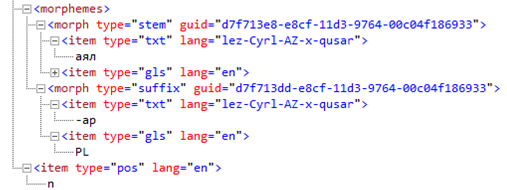
\includegraphics{figs/FLExTxt0.png}
%\caption[Excerpt from FLExText XML format]{This FLExText XML format excerpt shows the morpheme breaks of one word consisting of a root morpheme followed by a plural suffix.}
%\label{fig:FLExTxt}
%\end{figure}

\begin{table}[h!]
\begin{center}
\begin{tabular}{lcccc}
\bf Label & \bf Precision & \bf Recall & \bf F$_1$& \bf Instances \\
\hline
stem &    0.98    &    0.97 &    0.97 &    127 \\
AOR    &    0.93    &    1.00 &    0.97 &    14 \\
FOC    &    1.00    &    1.00 &    1.00 &    10 \\
OBL &    0.75    &    0.67 &    0.71 &    9 \\
GEN    &    0.67    &    0.40 &    0.50 &    5 \\
ERG    &    0.67    &    0.40 &    0.50 &    5 \\
DAT    &    1.00    &    1.00 &    1.00 &    4 \\
NEG    &    1.00    &    0.75 &    0.86 &    4 \\
PTP    &    0.80    &    1.00 &    0.89 &    4 \\
SBST &    1.00    &    1.00 &    1.00 &    3 \\
IMPF &    1.00    &    1.00 &    1.00 &    2 \\
PERF &    1.00    &    1.00 &    1.00 &    2 \\
ELAT &    1.00    &    1.00 &    1.00 &    1 \\
SUPER &    1.00    &    1.00 &    1.00 &    1 \\
\hline
total/avg affixes & 0.84 & 0.80 & 0.82 & 64\\
total/avg all &    0.92 &    0.87 &    0.90 & 191 \\
\end{tabular}
\caption[Segmentation and Glossing Pilot Study Gloss Labels]{
Results per gloss label. CRF-only. 
%(ERG = ergative case, AOR = aorist tense, etc.)
}
\label{tab:pilot1CRFResults}
\end{center}
\end{table}

Three models were trained and compared. The CRF and SVM models were used as described in the previous section but the third model was an LSTM-based sequence-to-sequence neural network \citep{sutskever2014} with attention \citep{bahdanau2014}. 
%All characters that are not part of a word (e.g. digits and punctuation) were eliminated in pre-processing. Incorrect glosses were identified and corrected by printing out tags and allowing a linguist to spot check the annotations to see if, for example, the distribution of POS tags appeared normal.
%Every word had been tagged for part of speech. Since it seemed reasonable to expect that a native speaker educated in another language could quickly learn to recognize basic parts of speech in her own language, the feature-based models assumed that POS tags exist in language documentation and description data. (I have since found that this expectation is not reasonable for language documentation and description corpora. Therefore, POS tags will not be assumed to exist in the dissertation.) The Lezgi data included two POS tags for categories that are not basic. Participles and demonstrative pronouns are more abstract categories but their distinctions are kept simply because they had already been very consistently annotated. 
%All but the neural model assume that (1) the data has been analyzed in FLEx, as shown in Figure \ref{fig:FLEX}, and exported as a FlexText XML format, shown in Figure \ref{fig:FLExTxt}, (2) words have been tagged for part of speech, (for the case study - verb, participle, adjective, adverb, noun/proper noun, particle, pronoun, demonstrative pronoun, and postposition), (3) morpheme segmentation and glosses are consistent, and (4) all affixes, but not stems, are glossed. 
The overall accuracy of morpheme boundary and gloss prediction was compared across the three systems. Table \ref{tab:pilot1Results} shows the results on a held-out test set. Joint segmentation and glossing with the CRF produced the best results. All three models performed near or above the target of 60-80\% F$_1$-score.

Ten texts containing a little over 3,000 words were excerpted from the corpus and formatted for training. The output labels for the CRF and LSTM were identical. There was one label per character and a BIO tag was included for both models but they did not include morpheme segments (e.g. a m $\longrightarrow$ B-be I-be). For the SVM model, the predicted morphemes were reconstructed by concatenating letters based on their BIO tag. All models were fed one sentence per line. Since inflectional morphemes are a closed class the models were trained to gloss them. Stems, however, being an open class, were glossed merely as ``stem''. Table \ref{tab:pilot1CRFResults} shows the CRF's joint accuracy for prediction of boundaries and glosses for each possible gloss. 

%shows that model's ability to produce reasonable results with limited training data. 
%The pilot study indicates that the typical IGT output of a language documentation and description project is sufficient to support integration of machine learning into segmenting and glossing--at least as far as the 3,000 tokens available Lezgi  are representative of a typical language documentation and description project. The most acute issue is the reduction of accuracy when predicting stems compared to when predicting affixes, as shown in the last line of Table \ref{tab:pilot1CRFResults}. The classifier is, however, adept at splitting affixes from stems, and this in itself would be helpful assistance to human annotators. All but a handful of affixes are identified with very high accuracy. These exceptions indicate that limited data may not be sufficient for languages with extensive allomorphy. 

%It is crucial to test the three models on other languages, especially a language with more complicated morphophonology. The features used for the feature-based models proved sufficient for Lezgi and expanding to other languages might uncover more general linguistic features that would maintain high accuracy for more languages. A neural model could plausibly be improved by data augmentation techniques using artificially generated training data that have proved successful in low-resource settings. 